\documentclass[border=10pt]{standalone}
\usepackage{pgfplots}
\pgfplotsset{compat=1.18}

\begin{document}
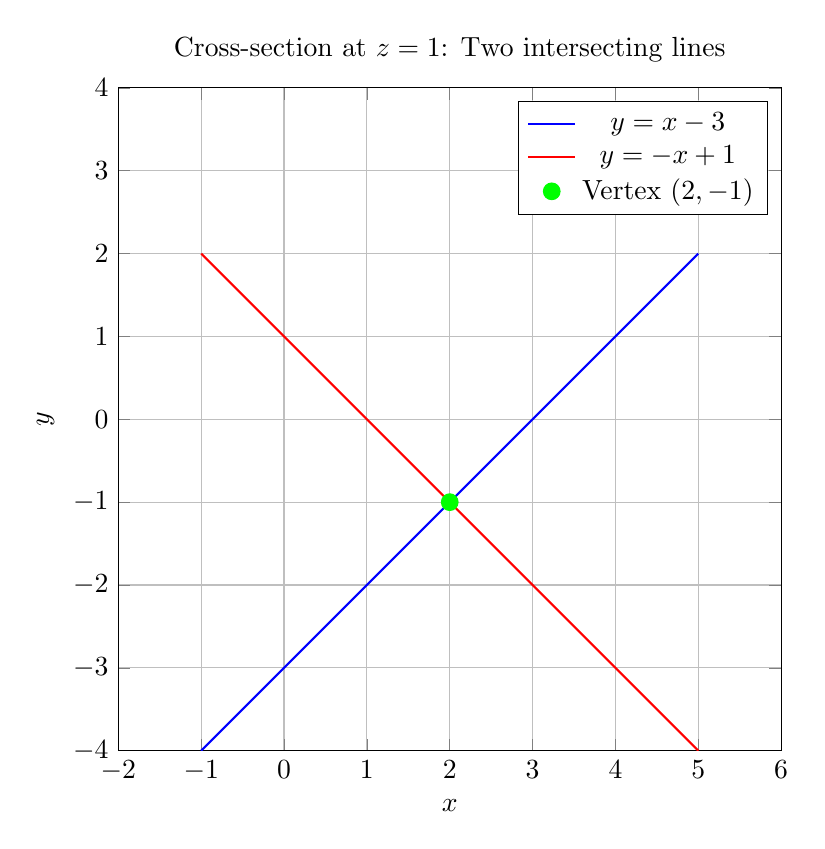
\begin{tikzpicture}
\begin{axis}[
    width=10cm,
    height=10cm,
    xlabel=$x$,
    ylabel=$y$,
    title={Cross-section at $z=1$: Two intersecting lines},
    axis equal,
    grid=major,
    xmin=-1, xmax=5,
    ymin=-4, ymax=4,
]

% Line y = x - 3
\addplot[
    blue,
    domain=-1:5,
    thick,
] {x - 3};
\addlegendentry{$y = x - 3$}

% Line y = -x + 1
\addplot[
    red,
    domain=-1:5,
    thick,
] {-x + 1};
\addlegendentry{$y = -x + 1$}

% Vertex point
\addplot[
    only marks,
    mark=*,
    mark size=3pt,
    green,
] coordinates {(2, -1)};
\addlegendentry{Vertex $(2, -1)$}

\end{axis}
\end{tikzpicture}
\end{document}